

% *********************
% Infoga bild

% se Figur \ref{fig:stable}.

%\begin{figure}[H]
%  \includegraphics[width=165mm]{stabil.png}
%  \caption{Den slutliga versionen av kretsen i Logisim.}
%  \label{fig:stable}
%\end{figure}


% *************************************************************************
% *************************************************************************
% *************************************************************************
% *************************************************************************


Projektet är uppdelat i fem stora delar: priv\_imalloc, refcount, gc, memory och utilities. Det kändes som en naturlig uppdelning. Memory var från början från början kallad freelist, men ändrades sedan till att kallas för memory då den modulen hanterar allt som rör freelistan samt alloclistan (listan med allokerade objekt). Utilities skapades för att tillåta användning av boolean och för att komma åt refcounten (sparad som metadata).

De olika delarna är inte exakt lika stora och omfattande men är viktiga för att få en logisk struktur på projektet.

Vi delade upp programmet baserat på hur de olika delarna hänger ihop med varann. Vi försökte lyfta ut kod som används av flera moduler i separata block så vi slipper upprepad kod. Till exempel vill vi kunna använda chunklistorna i de flesta moduler. Vi tänkte också på att varje block skulle kunna skrivas oberoende av hur de andra såg ut, även om detta inte alltid var helt möjligt. På så sätt blev det lättare att skriva tester innan man började koda då man inte behövde tänka på hur miljön såg ut utanför ens egen modul.

I början tyckte vi att den “indelning” som stog i projektspecifikationen kändes relativt bra, dvs att dela upp minneshantering med alloc och free, referensräknaren och garbage collection i tre block, men valde sedan att dela upp det ytterligare, exempelvis lämpade sig inte delen med alloc och free att vara en egen del då den var så liten.



\begin{figure}[H]
  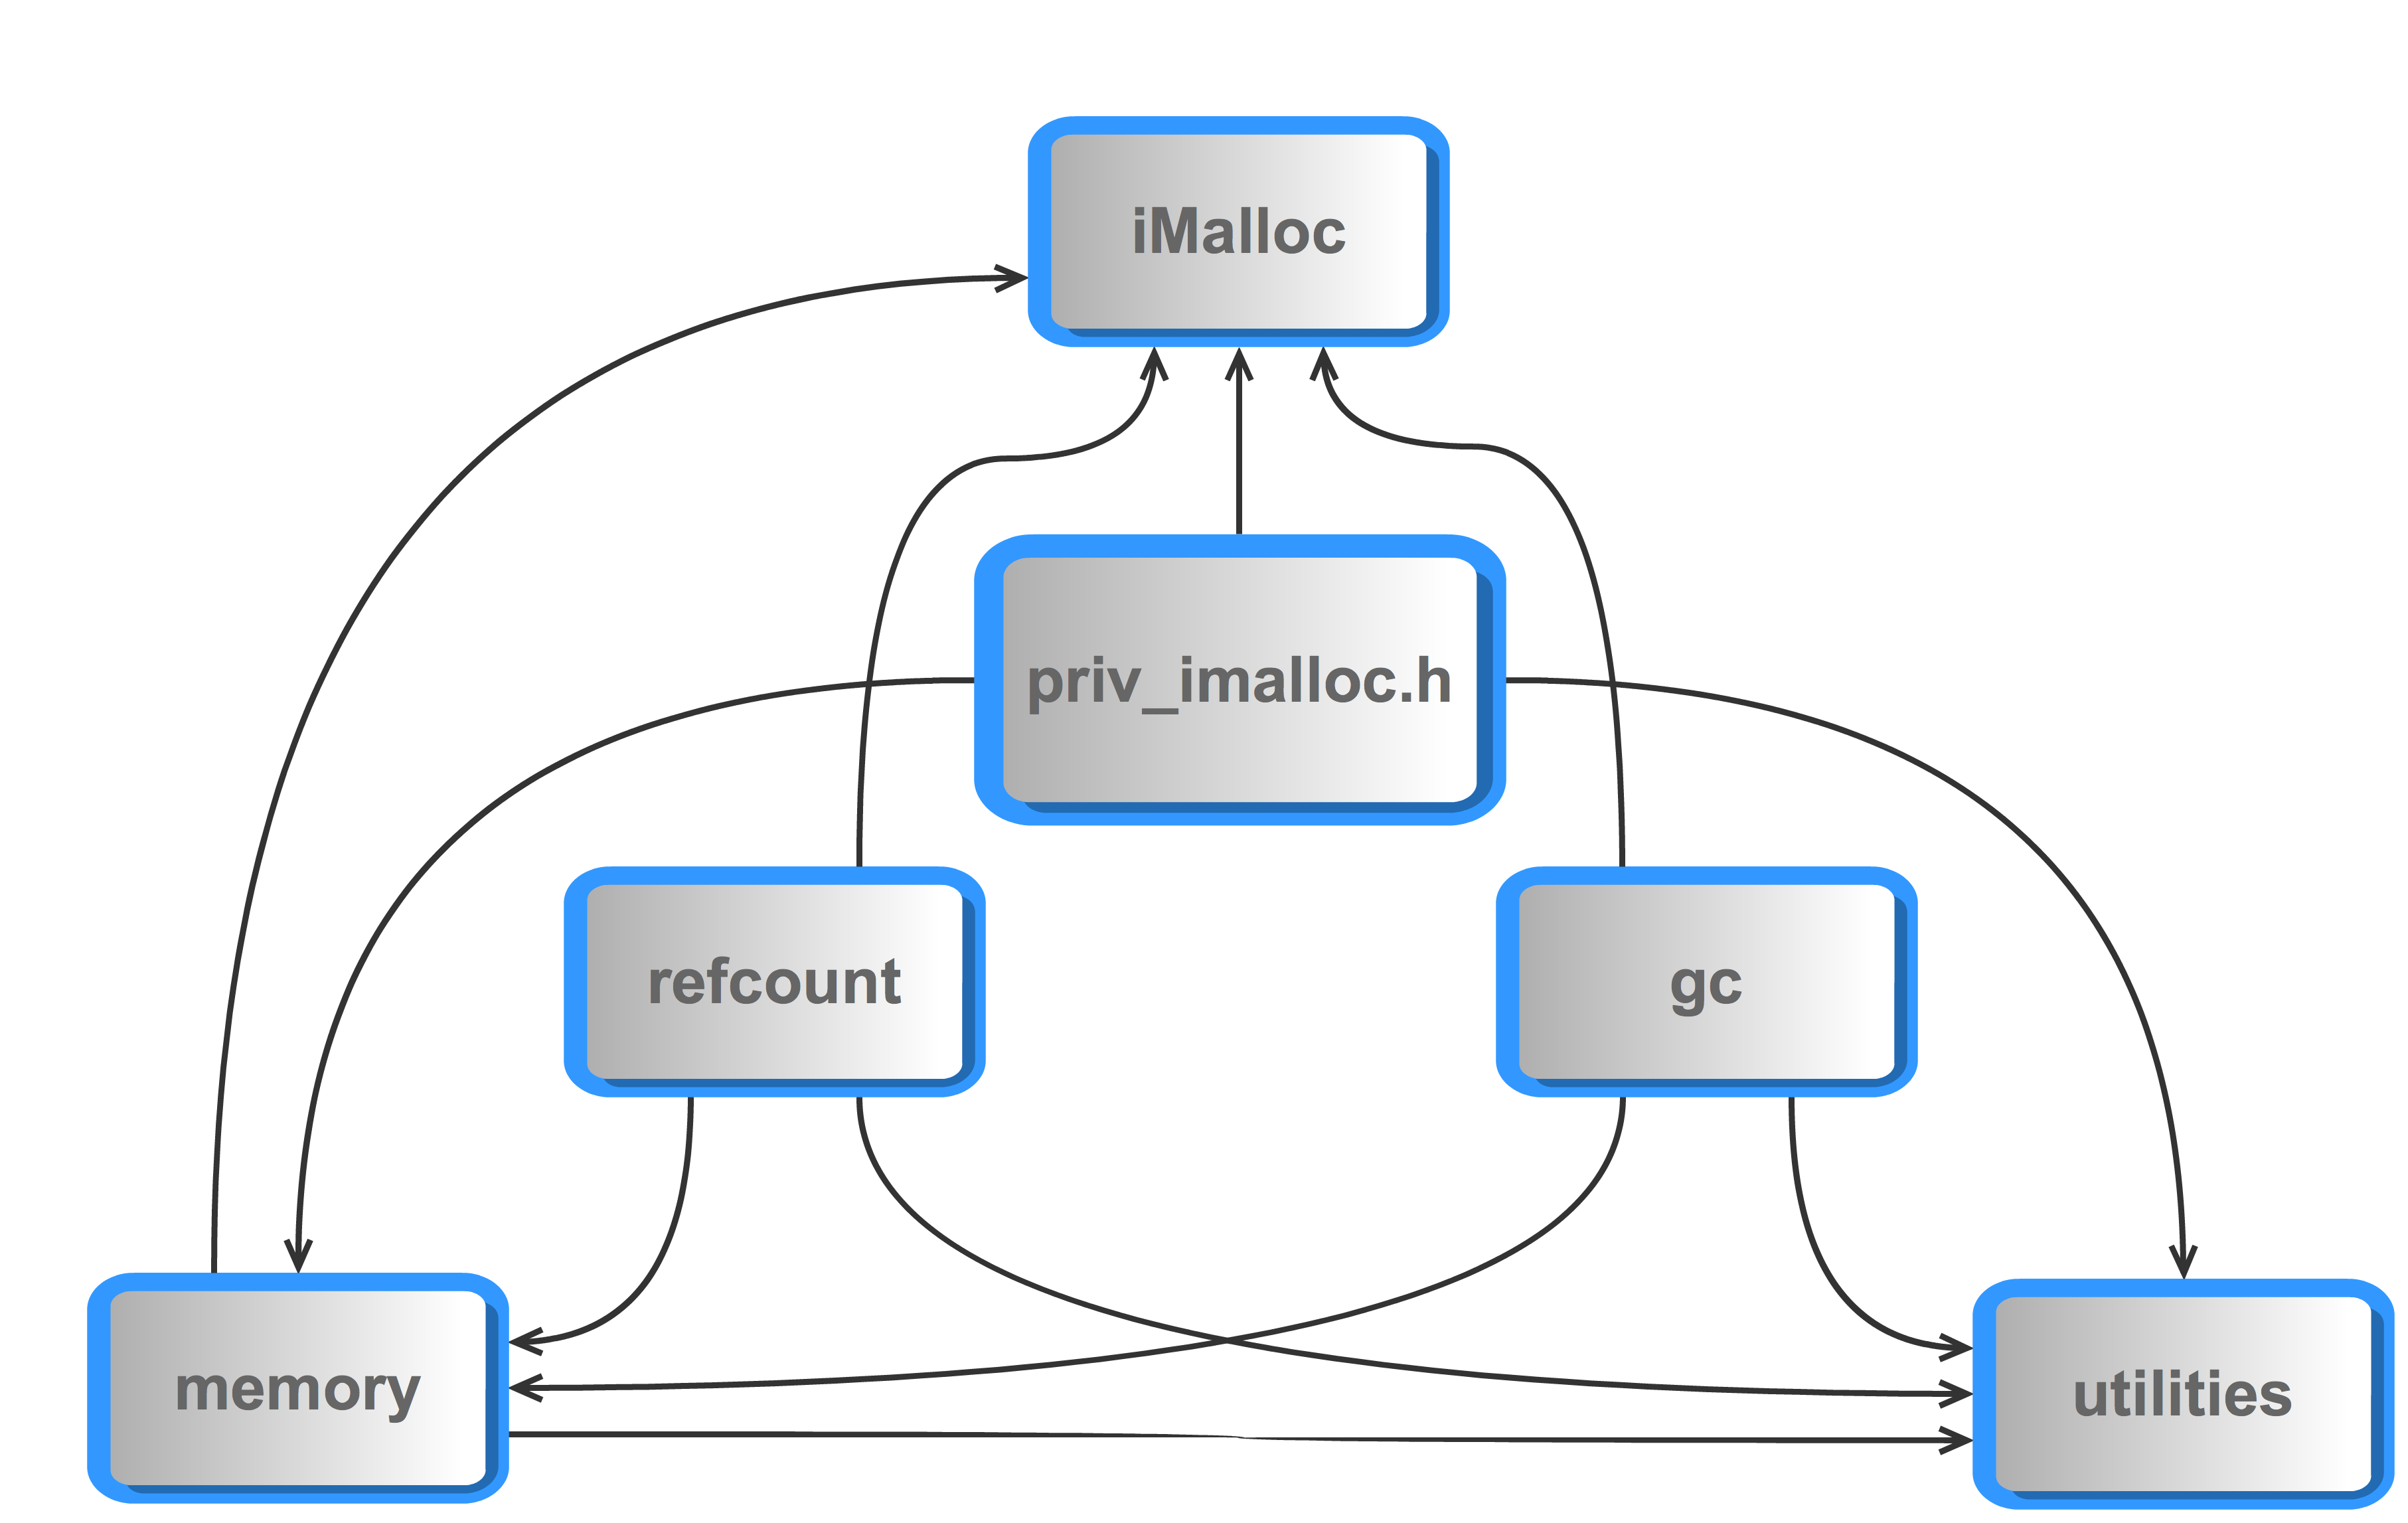
\includegraphics[width=\columnwidth]{images/design_overview.png}
  \caption{Den övergripande designen för programmet.}
  \label{fig:design_overview}
\end{figure}



Här nedan är ett flödesschema på lägre nivå, en mer detaljerad beskrivning av vad hjälpfunktionerna till priv\_imalloc gör och hur de kommunicerar med varandra.

manual, refcount och gc anropar alla varsin typ av alloc. I fallet för gc kan den anropa både typed Alloc eller managed Alloc, beroende på hur input-flaggorna ser ut. typed Alloc gör samma sak som managed Alloc bara att den första gör ett anrop till format för att få ut rätt storlek på formatsträngen.

Samtliga “special Allocs” använder sig av den universala iAlloc.


\begin{figure}[H]
  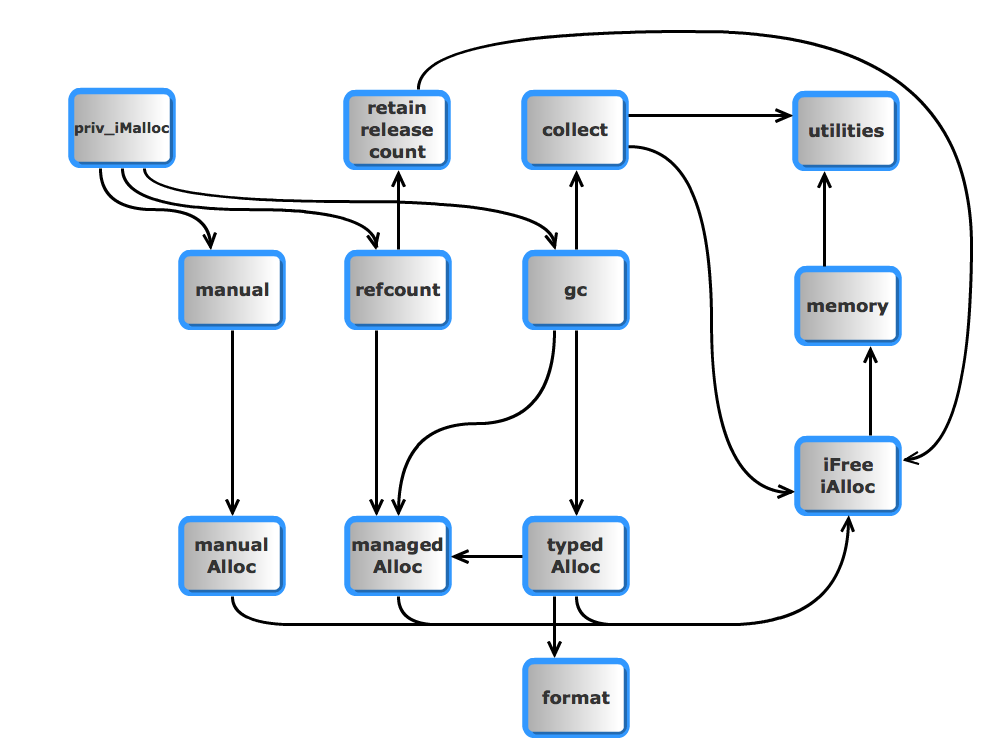
\includegraphics[width=\columnwidth]{images/design_depth.png}
  \caption{En mer djupgående beskrivning av vår design.}
  \label{fig:design_depth}
\end{figure}

